\documentclass{article}

% --- Import packages ---
\usepackage[utf8]{inputenc}
\usepackage{fancyhdr}
\usepackage{graphicx}
\usepackage[headheight=2cm,]{geometry}
\usepackage[most]{tcolorbox}
\usepackage{lipsum}
\usepackage{pgfplots}
\usepackage{xcolor}
\usepackage{multirow}

% --- Defining bibliography backend and package ---

\usepackage[backend=biber,defernumbers=true]{biblatex}
\addbibresource{Zdroje/Zdroje.bib}

% --- Defining new thicker hline ---

\makeatletter
\newcommand{\thickhline}{%
    \noalign {\ifnum 0=`}\fi \hrule height 1pt
    \futurelet \reserved@a \@xhline
}

% --- Defining a set of colors ---

\definecolor{brown}{RGB}{149,36,47}

% --- Set pgfplotsset ---
\pgfplotsset{compat=1.16}

% --- Define page styles ---
\pagestyle{fancy}
\fancyhf{}
\renewcommand{\headrulewidth}{0pt}
\fancyhead{}
\chead{\includegraphics{Images/School_Logo.png}}

% --- Define newtcolorbox environment ---
\newtcolorbox{lefttextpipe}{
	enhanced jigsaw,
    breakable=true,
    outer arc=0pt,
    arc=0pt,
    colback=white,
    rightrule=0pt,
    leftrule=2pt,
    toprule=0pt,
    top=0pt,
    right=-3pt,
    bottom=4pt,
    bottomrule=0pt,
    colframe=black,
    enlarge left by=15pt,
    width=\linewidth - 15pt,
    colframe=brown,
    enlarge left by=-20pt 
}

% --- Define variable file ---
\newcommand\Authors{Sofia Drahná Saakyan, Dominik Bálint}
\newcommand\Company{Proxy, a.s.}
\newcommand\TitleOfTheWork{\textbf{\Huge Strategický audit\\}\Company}
\newcommand\InformationOfTheWork{Právo v obchodních vztazích, dominik.balint@vsci.cz, sofia.drahna@vsci.cz}

% --- Define date format ---

\def\shortdateformat{\leavevmode\hbox{\twodigits\day.\twodigits\month.\the\year}}
\def\twodigits#1{\ifnum#1<10 0\fi\the#1}

% --- Define maketitle values ---
\author{\Authors}
\date{\InformationOfTheWork, \shortdateformat}
\title{\TitleOfTheWork}

% --- Begin the document ---
\begin{document}

\maketitle
\vspace*{5mm}
\tableofcontents
\listoffigures
\listoftables

\newpage

\thispagestyle{fancy}

\newcommand\PredstaveniSpolecnosti{PŘEDSTAVENÍ SPOLEČNOSTI Proxy, a.s.}
\begin{lefttextpipe}
	{\huge \PredstaveniSpolecnosti}
\end{lefttextpipe}
\phantomsection
\addcontentsline{toc}{section}{\PredstaveniSpolecnosti}

Předmětem podnikání společnosti je především \textit{daňové poradenství} a \textit{činnost účetních poradců, vedení účetnictví, vedení daňové evidence}. Společnost má okolo 60 zaměstnanců\footnote{V Merku je možné dohledat číslo 50 - 99 zaměstnanců.}\textsuperscript{, }\footfullcite{proxy_merk} a je lokalizována v České republice. Společnost je součástí většího holdingu PROXY Holding a.s.. Společnost je dělená na několik oddělení, z nichž každá se soustředí na specifickou oblast v rámci daňového a účetního poradentsví, každá z těchto oblastní má vlastního manažera. Obecné směřování společnosti je stanovováno představenstvem.\\

Společnost se pohybuje výhradně na českém trhu v oblastni daňové a účetní, jejímy klienty jsou subjekty, které v České republice vykonávají jakoukoli ekonomickou činnost v rámci které jsou povinny řídit se českými daňovými a účetnímy předpisy. Hlavní službou společnost Proxy, a.s. je tak poskytování služeb související právě s činnostmi týkající se daní a vedení účetnictví a jedná se tedy výhradně o účetní a daňovou společnost.

\section*{A. Současná vize a poslání podniku}
\label{sec:Vize a poslani}
\addcontentsline{toc}{subsection}{\nameref{sec:Vize a poslani}}

\subsection*{A.1 Poslání a mise společnosti}
\label{sec:Poslani}
\addcontentsline{toc}{subsubsection}{\nameref{sec:Poslani}}

Dle informací na webových stránkách společnosti je základní poslání a mise poskytování služeb na poli daňového poradenství, účetnictví, mzdové evidence a dalšího specializovaného poradenství\footfullcite{proxy_website}, především pro zahraniční investory vstupující na český trh a zjednodušit a zpřehlednit jim tam investici a fungování v České republice. 

\subsection*{A.2 Vize}
\label{sec:Vize}
\addcontentsline{toc}{subsubsection}{\nameref{sec:Vize}}

Vize společnosti spočívá především v tom, aby se stala partnerem pro své klienty a nadále je podporovala kvalifikovaným poradenstvím a to jak pro českou, tak i pro mezinárodní klientelu. Společnost se stala v roce 2004 součástí mezinárodní asociace poradenských firem HLB se sídlem v Londýně a nadále tak podporuje svojí vizi o kvalitní poradenské činnosti v dané oblasti\footfullcite{proxy_o_firme}.

\subsection*{A.3 Aktuální problémy}
\label{sec:Problemy}
\addcontentsline{toc}{subsubsection}{\nameref{sec:Problemy}}

%Problémy jsou příležitosti.

%Problém bude škláování a legislativní požadavky a jejich implementace a přenesení do procesů týkající se poradenství v oblasti daní a činnosti daňových poradců a účetních poradců a udržování knowledgebasu.

%Dále školení lidí, tato oblast je dost problematická, rovněž taky shánění lidí?

S ohledem na informace na webové stránce společnosti a finanční výkazy (viz analýza v části \textit{D. Současné cíle společnosti}) se společnost nepotýká s nedostatkem příležitostí a z nichž pramenícího zisku. Společnost je rentabilní a poptávka po jejích službách, vzhledem k výsledkům této analýzy, je vysoká.\\

Dle informací z Merku a Justice se společnost rovněž nepotýká s žádným právním problémem a není insolventní\footfullcite{proxy_merk}.\\

%\newpage

I s ohledem na výše uvedené informace je však možné vysledovat a odhadnout širší škálu problémů, se kterými se společnost této velikosti a významu potýká a ze své podstaty potýkat musí.\\

Nejzásadnější problémy lze rozdělit do několika kategorií:\\

\begin{itemize}
	\item reakce na poptávku a z toho vyplývající škálování,
	\item reakce na vnější faktory, především na měnící se legislativu,
	\item udržování knowledge base,
	\item roustoucí požadavky na kvalifikaci zaměstnanců\footnote{Zmíněno rovněž ve druhém bodu.},
	\item pandemie COVID-19,
	\item ostatní\footnote{Příkladem mohou být rostoucí náklady a mzdy.}.
\end{itemize}

\vspace*{5mm}

\newpage

\textbf{Reakce na poptávku, škálování}\\

Jako každá společnost musí i \textit{Proxy a.s.} reagovat na poptávku, pokud chce udržet svojí rentabilitu. Vzhledem k výsledku hospodaření za účetní období (viz graf níže) a vývoji počtu živnostenských oprávnění (viz reakce na konkurenci) lze dovodit, že poptávka po účetních službách dlouhodobě stoupá.

\begin{figure}[!htbp]
	\inputfile{Parts/IntroductionResources/CHART_Vyvoj_zisku}
	\caption[Výsledek hospodaření za účetní rok]{Výsledek hospodaření za účetní rok\protect{\footfullcite{proxy_merk}}}
	\label{fig:Vysledek hospodareni}
\end{figure}

Vzhledem ke zmíněnému růstu výsledků za sledovaná období lze dovodit, že Proxy na tento problém reaguje adekvátně a dokáže ho přeměnit na příležitost.\\

Důležité je však dodat, že nemáme informace týkající se výsledku hospodaření za rok 2020 a za rok 2021\footnote{Autoři jsou si vědomi, že ke dni vzniku této práce nenastala pro subjekt zákoná povinnost uveřejnit účetní závěrku ve sbírce listin.}, neboť listyny dosud nebyly vloženy do sbírky listin\footfullcite{proxy_justice}. Z tohoto důvodu není možné se stoprocentní jistodou dovodit stejné závěry i pro rok 2020 a 2021, z historického vývoje není rovněž možné se stoprocentní jistotou vycházet vzhledem k probíhající pandemii i jími podnícenými změnami na trhu.\\

\newpage

 Vzhledem k výsledkům hospodaření za roky předcházející a stále rostoucímu počtu živnostenských oprávnění v daném oboru se autoři, i přes výše zmíněnou problematiku, domnívají, že lze důvodně dovodit, že trend růstu výsledku hospodaření a tedy přímý výsledek využitých příležitostí by měl mít i pro rok 2020 (Viz kapitola \textit{C. Životní cyklus firmy}) a 2021 rostoucí charakter\footnote{Viz problematika popsaná níže v části Pandemie COVID-19.}. Minimálně za období 2014 až 2019 lze vyhodnotit, že reakce na poptávku ze strany společnosti je více než adekvátní, a že společnosti se podařilo dosáhnout a udržet dlouhodobý růst.\\

%Nemáme však info za rok 2020 a 2021 vzhledem k výsledku hospodaření, ale vzhledem ke stále rostoucímu počtu podnikatelů v dané oblastni (živnostenských oprávnění) lze důvodně dovodit, že poptávka neklesá. Minimálně za období 2014 - 2019 lze vyhodnotit, že reakce na poptávku ze strany společnosti je více než adekvátní a že společnosti se podařilo udržet dlouhodobý růst.\\

%\newpage

\textbf{Reakce na konkurenci}\\

Jako káždá společnost je potřeba reagovat na konkurenci.

\begin{figure}[!htbp]
	\inputfile{Parts/IntroductionResources/CHART_Ziv_number_in_time}
	\caption[Počet živností]{Počet živností\footfullcite{noauthor_pocty_nodate}}
	\label{fig:Pocet zivnosti}
\end{figure}

S ohledem na rostoucí počet živností v průběhu roku, se tento bod musí stát zájmem strategického řízení společnosti.\\

\textbf{Reakce na měnící se legislativu}\\

Společnost se rovněž musí potýkat neustále s měnící se legislativout, a to ať už týkající se samotné činnosti, či předpokladů, které společnost musí splňovat k tomu, aby činnost jako takovou mohla vykonávat\footnote{Jako příklad mohou sloužit zákony č. 586/1992 Sb., či zákon č. 235/2004 Sb., které souhrnně prošli v posledních letech velkým množstvím novelizací.}.\\

\textbf{Udržování knowledge base}\\

\vspace*{-1mm}

I vzhledem k předchozímu bodu a neustále se měnícím podmínkám na trhu si musí společnost udržovat kvalitní knowledge base, který musí být co nejaktuálnější, aby mohla svižně reagovat na jakékoliv změny v oboru. Musí tedy průběžně přizpůsobovat procesy a metodologii s ohledem na tyto změny v daňových a účetních normách a nejen v těch, jedná se proto o zásadní externí faktor.\\


%škálování vzhledem k dlouhodobému ekonomickému růstu a větší poptávce po daňovém a účetním poradenství, toto lze dovodit s ohledem jejich stránku kde chtějí studenty a mají permanentně vyvěšené pracovní nabídky, ČSÚ a vývoj počtu podnikatelů v dané oblastni a růstu vykazovanému v účetniství. Lze soudit ze statistik MPO odkaz za sledované období čtvrtého, respektive třetího kvartálu od roku 2016 až 2021

%Ahoj.
%Data2 2

%Hello?
%\inputfile{Parts/IntroductionResources/CHART_Vyvoj_zisku}

%\begin{center}
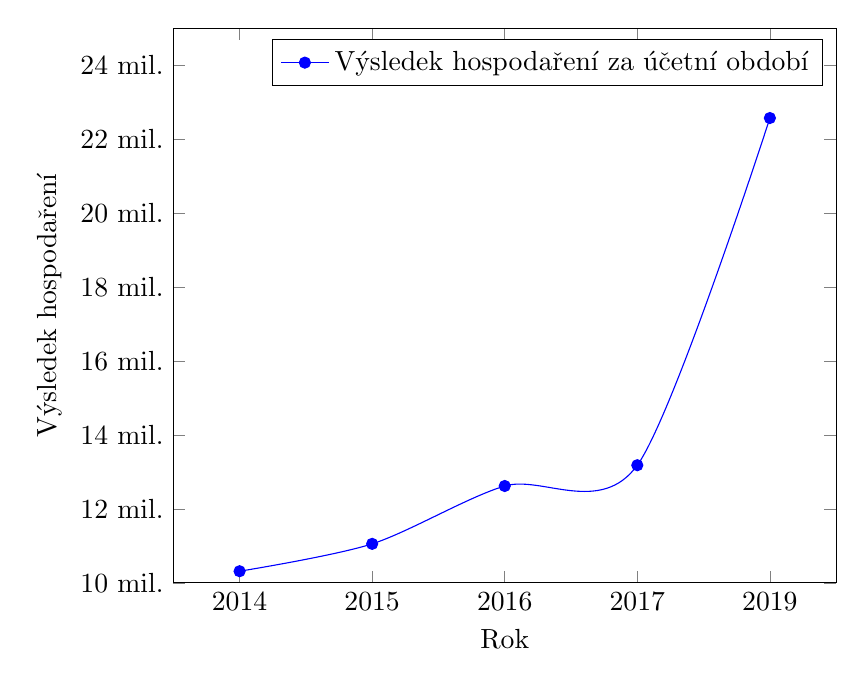
\begin{tikzpicture}
	\begin{axis}[
		width=10cm,
    	xlabel=Rok,
    	ylabel=Výsledek hospodaření,
    	xmin=0, xmax=100,
    	ymin=10, ymax=25,
    	xtick={10,30,50,70,90},
    	xticklabels={2014,2015,2016,2017,2019},   % <---
    	ytick={10,12,...,24},
    	yticklabels={10 mil., 12 mil., 14 mil., 16 mil., 18 mil., 20 mil., 22 mil., 24 mil.}
            ]
		\addplot[smooth,mark=*,blue] 
			plot coordinates {
    			(10,10.314)
    			(30,11.054)
    			(50,12.619)
    			(70,13.181)
    			(90,22.571)
			};
		\addlegendentry{Výsledek hospodaření za účetní období}

	\end{axis}
\end{tikzpicture}
\end{center}

%\input{Parts/IntroductionResources/Diagram}

%Taky bych sem měl zařadit analýzu, respektive graf rostoucích příjmů - pak rovněž odkázat na část, kde řeším příjmy v analýze.

%Lze možná dooknce usoudit, že nárůst je způsobený i růstem příležitostí během COVIDU 19 a sním spojené nutnosti postarat se o daně a účetnivtví.


 %a udržování knowledge basu a přizpůsobování procesů neustále se měnícím požadavkům na daňové a účetní, respektive finanční poradenství a povinnosti s ním související v českém právním prostoru, jedná se tedy o zásadní externí faktor.\\
 
\textbf{Pandemie COVID-19}\\

\vspace*{-1mm}

Společnost tuto problematiku uznává v rámci Účetní závěrky za rok 2019, ta specificky zmiňuje:\\

\vspace*{-1mm}

\textit{Koncem roku 2019 se poprvé objevily zprávy z Číny týkající se COVID-19 (koronavirus). V prvních měsících roku 2020 se virus rozšířil do celého světa a způsobil rozsáhlé ekonomické škody. I když v době zverejnení této účetní závěrky vedení společnosti nezaznamenalo významný pokles prodeje, situace se neustále mění, a proto nelze předvídat budoucí dopady této pandemie na činnost společnosti. Vedení společnosti bude pokračovat v monitorování potenciálního dopadu a podnikne veškeré možné kroky ke zmírnění jakýchkoliv negativních účinků na společnost a její zaměstnance.}\footfullcite[Účetní závěrka za rok 2019]{proxy_justice}

\subsection*{A.4 Green deal}
\label{sec:Green deal}
\addcontentsline{toc}{subsubsection}{\nameref{sec:Green deal}}

Společnost Proxy a.s., se ve svých veřejně publikovaných dokumentech společenské odpovědnosti jí vyplývající z jejího postavení vzhledem k životnímu prostředí, a nejenom jemu, nevěnuje\footnote{Autoři vycházejí především z veřejně dostupných informací společnosti a dokumenty a články, které společnost publikovala.}.\\

%Carbon footprint - office, auta etc.

\vspace*{-1mm}

Vzhledem k tomu, že se společnost problémem aktivně nazabývá, což je vzhledem ke stále více sílícím společneským tendencím tuto problematiku řešit problematické, autoři kladou v závěru v projektové části doporučení týkající se zavedení procesů směřující k větší společenské odpovědnosti ve vztahu k udržení přírody a redukce tvorby emisí a dalších pro přírodu negativních dopadů spojených s provozem činnosti subjektu.\\

\vspace*{-1mm}

I vzhledem k faktu, že strategický audit se nevěnuje výrobní společnosti, která je vhledem k povaze své činnosti ze své podstaty mnohem větším znečišťovatelem, je iluzorní předpokládat, že společnost poskytující služby nevyprodukuje svojí činností jakékoliv emise, a že nemá jakékoliv další negativní dopady na životní prostředí\footfullcite{anon_sustainable_2013}\textsuperscript{,}\footfullcite{anon_using_2011}. Emise společnost, ať už přímo, či nepřímo, produkuje nejen díky provozování faktických kancelářských prostor, ale i díky provozování flotily automobilů a zaměstnaneckou činností\footnote{Příkladem je doprava do místa výkonu činnosti zaměstnanců, používání elektroniky k výkonu činnosti a používání dalších hmotných věcí a s tím spojenou nutností jejich produkce a likvidace.}. 


%Jako příklad negativního dopadu provozu činností, které svojí povahou nejsou přímo výrobní lze uvést například je možné uvést potřebu redukce negativního dopadu v oblastni procurementu kancelářských potřeb, vycházejících 

%Green deal je, odkaz, vztah společnosti ke green dealu je, blabla odkaz. Moc nemusí řešit green deal, nejsou výrobní společnost, která by generovala velké množství znečištění.

\section*{B. Identifikace procesu strategického řízení}
\label{sec:Identifikace procesu strategickeho rizeni}
\addcontentsline{toc}{subsection}{\nameref{sec:Identifikace procesu strategickeho rizeni}}

Společnost je vlastněna společností Proxy Holding a.s. z 90\%\footfullcite{noauthor_verejny_nodate}\textsuperscript{,}\footnote{Zbytek akcií zřejmě vlastní drobní akcionáři, tato informace bohužel není veřejně dostupná.}, proto přebírá jeho strategii, která se rovněž týká strategie celého holdingu.\\

Strategie jako taková je tedy formulována subjektem Proxy Holding a.s., společnost Proxy a.s. strategii přebírá. Strategie existuje v podobě dlouhodobého plánování o směřování organizace, které je udržováno představenstvem. Společnost jí průběžně aktualizuje, informace o tom zda má společnost k této aktivitě vytvořené směrnice společnost bohužel nepublikuje.\\

Jak již bylo řečeno společnost je součástí širšího holdingu, který zahrnuje i další subjekt, a to společnost Proxy - Audit s.r.o., společnosti jsou velice propojené, a to do té míry, že společnost prezentuje všechny dílčí aktivity pod jednou střechou\footfullcite{proxy_website}.\\

Tvorba strategie je tak omezena potřebou dalších subjektů, to samozřejmě představuje řadu omezení pro tvorbu celkové strategie, která má tak mnoho omezujícíh faktorů vzhledem k zájmu celé skupiny.\\

Na závěr je důležité říci, že společnost je v relativně stabilním businessu a těší se dlouhodobému růstu, společnost pokrývá téměř všechny oblasti v dané kategorii služeb, potřeba zásadních revizí strategických plánů tak není tak častá. Společnost se tedy zaměřuje především na operativní plánování.\\

Společnost je procesně řízena v klasickém hierarchickém pojetí. Má však dobře vydefinované procesy a metodologii vzhledem k nárokům trhu a legislativním požadavkům. Společnost je tedy procesně zralá\footnote{Bližší informace k organizační struktuře, řízení kompetencí a informačnímu systému obsahuje kapitola \textit{D. Organizační struktura a kultura podniku}.}.\\

\textbf{Interní stakeholders}\\

%Sem napíšu že nevím, takže píšu ostatní, jinak poznamenávám, že to bude hlavně z 90 \% Proxy Holding a.s., a z 10 \% drobní akcionáři.\\

Společnost své stakeholdery přímo nepublikuje, do interních stakeholderů společnosti však můžeme zařadit především Proxy Holding a.s., především díky zmíněnému 90\% podílu, dále zaměstnance a management.\\

K interním stakeholderům přistupuje společnost jako k subjektům, kteří se podílejí na provozu společnosti dle pozice, přesné stanovení přísupu bohužel autorům není známé.\\

\textbf{Externí stakeholders}\\

%Sem napíšu obecné externí stakeholdery.\\

Do externích stakeholderů autoři řadí drobné akcionáře celkově držící 10\% podíl, zákazníky, dodavatelé, věřitelé a partnerské subjekty.\\

K externím stakeholderům společnost přistupuje zodpovědně, což je vidět nejenom na jejím ratingu\footnote{Viz Merk.}, ale rovněž na absenci negativních informací o společnosti. Přesně stanovený přístup bohužel autorům není znám.\\

%Úplně nemají, jenom základy podle kterých se řídí a jsou aktualizovány vedením společnosti, jsou v relativně stabilním businessu a pokrývají všechny oblasti v dané kategorii v četně auditu, takže úplně nepotřebují strategický plán.

%Majá spíš operativní - na koho, kdy a jak se zaměří - maj i svojí klientelu, takže nepotřebují akvizici tak zásadně.

\section*{C. Popis současného obchodního modelu}
\label{sec:Popis soucasneho obchodniho modelu}
\addcontentsline{toc}{subsection}{\nameref{sec:Popis soucasneho obchodniho modelu}}

Současný model se soustředí na poskytování služeb v oblasti daňové, účetní a auditorské (v rámci jiné společnosti).\\

Investiční náklady bohužel nejsou autorům známé.\\

\noindent\textbf{Analýza obchodního modelu:}

\begin{enumerate}
	\item komu slouží: subjektům, kteřé na území České republiky provozují jakoukoli činnost, která jim zakládá povinnosti řídit se českými právními předpisy týkajícími se daňového a účetního práva, v konečném důsledkům pak také samozřejmě finálním příjemcům,
	\item co poskytuje: finanční služby, specificky služby účetní, daňové a auditorské, společnost rovněž publikuje články a pořádá školení,
	\item jak vydělává peníze, jaké používá metody: přímým poskytováním služeb, společnost má stálou klientelu a akvizice probíhá organicky,
	\item jak se odlišuje a udržuje konkurenční výhodu: dobré jméno na trhu, kvalita a dlouhé působení na trhu,
	\item jak poskytuje svojí službu: prostřednictvím poradců.
\end{enumerate}

\newpage

Tabulka sledovaných hodnot z výkazu zisků a ztrát se zpracovaným cashflow:\\

\begin{table}[!hbtp]
\centering
\begin{tabular}{|l|ccccc|}
\hline
\multicolumn{1}{|c|}{} & \multicolumn{5}{c|}{Sledované období} \\ \cline{2-6} 
\multicolumn{1}{|c|}{\multirow{-2}{*}{Sledované položky}} & \multicolumn{1}{c|}{2015} & \multicolumn{1}{c|}{2016} & \multicolumn{1}{c|}{2017} & \multicolumn{1}{c|}{2018} & 2019 \\ \hline
PS Cash & \multicolumn{1}{c|}{13 678} & \multicolumn{1}{c|}{13 917} & \multicolumn{1}{c|}{16 423} & \multicolumn{1}{c|}{15 857} & 16 181 \\ \hline
\rowcolor[HTML]{C0C0C0} 
 & \multicolumn{1}{c|}{\cellcolor[HTML]{C0C0C0}} & \multicolumn{1}{c|}{\cellcolor[HTML]{C0C0C0}} & \multicolumn{1}{c|}{\cellcolor[HTML]{C0C0C0}} & \multicolumn{1}{c|}{\cellcolor[HTML]{C0C0C0}} &  \\ \hline
EBT & \multicolumn{1}{c|}{13 792} & \multicolumn{1}{c|}{15 920} & \multicolumn{1}{c|}{16 413} & \multicolumn{1}{c|}{22 682} & 28 203 \\ \hline
Odpisy (+) & \multicolumn{1}{c|}{1762} & \multicolumn{1}{c|}{1734} & \multicolumn{1}{c|}{1873} & \multicolumn{1}{c|}{1706} & 1696 \\ \hline
Úroky (+/-) & \multicolumn{1}{c|}{0} & \multicolumn{1}{c|}{0} & \multicolumn{1}{c|}{0} & \multicolumn{1}{c|}{0} & 0 \\ \hline
$\Delta$ Zásoby (+/-) & \multicolumn{1}{c|}{89} & \multicolumn{1}{c|}{-53} & \multicolumn{1}{c|}{-24} & \multicolumn{1}{c|}{144} & 123 \\ \hline
$\Delta$ Pohledávky   (+/-) & \multicolumn{1}{c|}{1021} & \multicolumn{1}{c|}{1340} & \multicolumn{1}{c|}{-1 293} & \multicolumn{1}{c|}{2 879} & -14 \\ \hline
$\Delta$ Závazky   (+/-) & \multicolumn{1}{c|}{-29} & \multicolumn{1}{c|}{1468} & \multicolumn{1}{c|}{5432} & \multicolumn{1}{c|}{-1238} & 3604 \\ \hline
Zaplacená daň (-) & \multicolumn{1}{c|}{-2738} & \multicolumn{1}{c|}{-3301} & \multicolumn{1}{c|}{-3 232} & \multicolumn{1}{c|}{-4 619} & -5 632 \\ \hline
Provozní CF & \multicolumn{1}{c|}{13 897} & \multicolumn{1}{c|}{17 108} & \multicolumn{1}{c|}{19 169} & \multicolumn{1}{c|}{21 554} & 27 980 \\ \hline
\rowcolor[HTML]{C0C0C0} 
 & \multicolumn{1}{c|}{\cellcolor[HTML]{C0C0C0}} & \multicolumn{1}{c|}{\cellcolor[HTML]{C0C0C0}} & \multicolumn{1}{c|}{\cellcolor[HTML]{C0C0C0}} & \multicolumn{1}{c|}{\cellcolor[HTML]{C0C0C0}} &  \\ \hline
Nákup fixních aktiv (-) & \multicolumn{1}{c|}{0} & \multicolumn{1}{c|}{-384} & \multicolumn{1}{c|}{0} & \multicolumn{1}{c|}{-60} & -502 \\ \hline
Půjčky ve skupině (+/-) & \multicolumn{1}{c|}{0} & \multicolumn{1}{c|}{0} & \multicolumn{1}{c|}{0} & \multicolumn{1}{c|}{0} & 0 \\ \hline
Investiční CF & \multicolumn{1}{c|}{0} & \multicolumn{1}{c|}{-384} & \multicolumn{1}{c|}{0} & \multicolumn{1}{c|}{-60} & -502 \\ \hline
\rowcolor[HTML]{C0C0C0} 
 & \multicolumn{1}{c|}{\cellcolor[HTML]{C0C0C0}} & \multicolumn{1}{c|}{\cellcolor[HTML]{C0C0C0}} & \multicolumn{1}{c|}{\cellcolor[HTML]{C0C0C0}} & \multicolumn{1}{c|}{\cellcolor[HTML]{C0C0C0}} &  \\ \hline
Zvýšení ZK (+) & \multicolumn{1}{c|}{0} & \multicolumn{1}{c|}{0} & \multicolumn{1}{c|}{0} & \multicolumn{1}{c|}{0} & 0 \\ \hline
Bankovní úvěry (+) & \multicolumn{1}{c|}{0} & \multicolumn{1}{c|}{0} & \multicolumn{1}{c|}{0} & \multicolumn{1}{c|}{0} & 0 \\ \hline
Splátky bankovních úvěrů (-) & \multicolumn{1}{c|}{0} & \multicolumn{1}{c|}{0} & \multicolumn{1}{c|}{0} & \multicolumn{1}{c|}{0} & 0 \\ \hline
Emitované dluhopisy (+) & \multicolumn{1}{c|}{0} & \multicolumn{1}{c|}{0} & \multicolumn{1}{c|}{0} & \multicolumn{1}{c|}{0} & 0 \\ \hline
Vyplacené dluhopisy (-) & \multicolumn{1}{c|}{0} & \multicolumn{1}{c|}{0} & \multicolumn{1}{c|}{0} & \multicolumn{1}{c|}{0} & 0 \\ \hline
Finanční CF & \multicolumn{1}{c|}{0} & \multicolumn{1}{c|}{0} & \multicolumn{1}{c|}{0} & \multicolumn{1}{c|}{0} & 0 \\ \hline
\rowcolor[HTML]{C0C0C0} 
 & \multicolumn{1}{c|}{\cellcolor[HTML]{C0C0C0}} & \multicolumn{1}{c|}{\cellcolor[HTML]{C0C0C0}} & \multicolumn{1}{c|}{\cellcolor[HTML]{C0C0C0}} & \multicolumn{1}{c|}{\cellcolor[HTML]{C0C0C0}} &  \\ \hline
$\Delta$ Cash (+/-) & \multicolumn{1}{c|}{13 917} & \multicolumn{1}{c|}{16 423} & \multicolumn{1}{c|}{15 857} & \multicolumn{1}{c|}{16 181} & 23 618 \\ \hline
\rowcolor[HTML]{C0C0C0} 
 & \multicolumn{1}{c|}{\cellcolor[HTML]{C0C0C0}} & \multicolumn{1}{c|}{\cellcolor[HTML]{C0C0C0}} & \multicolumn{1}{c|}{\cellcolor[HTML]{C0C0C0}} & \multicolumn{1}{c|}{\cellcolor[HTML]{C0C0C0}} &  \\ \hline
KS Cash & \multicolumn{1}{c|}{27 575} & \multicolumn{1}{c|}{30 641} & \multicolumn{1}{c|}{35 592} & \multicolumn{1}{c|}{37 351} & 43 659 \\ \hline
\end{tabular}
\caption[Přehled cash flow za posledních 5 let]{Přehled cash flow za posledních 5 let\footfullcite[Účetní závěrky za roky 2015 - 2019]{proxy_justice}}
\label{tab:Prehled cash flow}
\end{table}

%Společnost Proxy a.s. vykazuje pozitivní cash flow, kromě roku 2016, kdy za sledované období došlo k poklesu. Cash flow má dlouhodobě stoupající tendenci.

Společnost Proxy a.s. vykazuje pozitivní \textbf{provozní cash flow}, které má stoupající tendenci.\\

Společnost dále vykazuje dlouhodobě záporné, nebo nulové \textbf{investiční cash flow}, což vzhledem k povaze tohoto ukazatele neznamená problém, neboť pořízená aktiva mohou do budoucna generovat vyšší zisk a vyšší provozní cash flow.\\

\textbf{Finanční cash flow} je za celé sledované období nulové.\\

Z výše přiloženého cash flow autoři nevnímají jakékoliv budoucní negativní tendence společnosti a považují jej za zcela v pořádku.\\

Další sledované hodnoty:\\

\begin{table}[!hbtp]
\begin{tabular}{l|l|l|l|l|l|}
\cline{2-6}
 & 2015 & 2016 & 2017 & 2018 & 2019 \\ \hline
\multicolumn{1}{|l|}{Tržby z prodeje výrobků a služeb} & 67108 & 72345 & 76690 & 92916 & 104449 \\ \hline
\multicolumn{1}{|l|}{Tržby za prodej zboží} &  &  &  &  &  \\ \hline
\multicolumn{1}{|l|}{Výkonová spotřeba} & 15771 & 17006 & 17362 & 24402 & 21735 \\ \hline
\multicolumn{1}{|l|}{Změna stavu zásob vlastní činnosti} & 89 & 53 & 24 & -144 & 123 \\ \hline
\multicolumn{1}{|l|}{Aktivace} &  &  &  &  &  \\ \hline
\multicolumn{1}{|l|}{Osobní náklady} & 34801 & 36779 & 39338 & 42901 & 49693 \\ \hline
\multicolumn{1}{|l|}{Úpravy hodnot v provozní oblasti} & 1805 & 1734 & 1873 & 1706 & 1696 \\ \hline
\multicolumn{1}{|l|}{Ostatní provozní výnosy} & 203 & 848 & 476 & 599 & 1171 \\ \hline
\multicolumn{1}{|l|}{Ostatní provozní náklady} & 765 & 1094 & 923 & 764 & 1445 \\ \hline
\multicolumn{1}{|l|}{Výnosy z dlouhodobého finančního majetku} &  &  &  &  &  \\ \hline
\multicolumn{1}{|l|}{Náklady vynaložené na prodané podíly} &  &  &  &  &  \\ \hline
\multicolumn{1}{|l|}{Výnosy z ostatního dlouhodobého   finančního majetku} &  &  &  &  &  \\ \hline
\multicolumn{1}{|l|}{Náklady související s ostatním   dlouhodobým majetkem} &  &  &  &  &  \\ \hline
\multicolumn{1}{|l|}{Výnosové úroky a podobné výnosy} & 3 & 0 & 0 & 0 & 33 \\ \hline
\multicolumn{1}{|l|}{Úpravy hodnot a rezervy ve fianční   oblasti} &  &  &  &  &  \\ \hline
\multicolumn{1}{|l|}{Nákladové úroky a podobné náklady} &  &  &  &  &  \\ \hline
\multicolumn{1}{|l|}{Ostatní finanční výnosy} & 49 & 5 & 217 & 121 & 106 \\ \hline
\multicolumn{1}{|l|}{Ostatní finanční náklady} & 719 & 612 & 1450 & 1307 & 2664 \\ \hline
\multicolumn{1}{|l|}{Daň z příjmů} & 2738 & 3301 & 3232 & 4619 & 5632 \\ \hline
\multicolumn{1}{|l|}{Převod podílu na výsledek hospodaření   společníkům} &  &  &  &  &  \\ \hline
\end{tabular}
\caption[Další sledované ukazatele]{Další sledované ukazatele\footnote{Tamtéž.}}
\label{tab:Dalsi sledovane ukazatele}
\end{table}

%\begin{figure}
%\inputfile{Parts/IntroductionResources/TABLE_Strategicke_ukazatele}
%	\caption{Test}
%	\label{tab:T}
%\end{figure}

\newpage

\section*{D. Současné cíle společnosti}
\label{sec:Soucasne cile spolecnosti}
\addcontentsline{toc}{subsection}{\nameref{sec:Soucasne cile spolecnosti}}

%Společnost proxy as vlastní společnost proxy holding as, má v něm 90\%, není tedy možné stanovit seznam akcionářů vzhledem k tomu, že zákon tuto povinnost ukládá při vlastníctví většího počtu akcií než 20\%.

%Společnost je součástí holdingu a asociace poradenských firem HLB se sídlem v Londýně.

\subsection*{D.1 Strategické}
\label{sec:Strategicke}
\addcontentsline{toc}{subsubsection}{\nameref{sec:Strategicke}}

Strategické cíle bohužel autoři nemají k dispozici, proto uvádí následující tabulku.\\

\begin{table}[!hbtp]
\centering
\begin{tabular}{|l|lllll|}
\hline
\multicolumn{1}{|c|}{\multirow{2}{*}{Strategický ukazatel}} & \multicolumn{5}{c|}{Vývoj v čase} \\ \cline{2-6} 
\multicolumn{1}{|c|}{} & \multicolumn{1}{c|}{2015} & \multicolumn{1}{c|}{2016} & \multicolumn{1}{c|}{2017} & \multicolumn{1}{c|}{2018} & \multicolumn{1}{c|}{2019} \\ \hline
NOPAT (EBIT*0,81) & \multicolumn{1}{l|}{11 172} & \multicolumn{1}{l|}{12 895} & \multicolumn{1}{l|}{13 295} & \multicolumn{1}{l|}{18 373} & 22 845 \\ \hline
Bilanční suma & \multicolumn{1}{l|}{31164} & \multicolumn{1}{l|}{36115} & \multicolumn{1}{l|}{33362} & \multicolumn{1}{l|}{36739} & 44179 \\ \hline
Tržby celkem & \multicolumn{1}{l|}{67108} & \multicolumn{1}{l|}{72345} & \multicolumn{1}{l|}{76690} & \multicolumn{1}{l|}{92916} & 104449 \\ \hline
Meziroční růst tržeb & \multicolumn{1}{l|}{3513} & \multicolumn{1}{l|}{5237} & \multicolumn{1}{l|}{4345} & \multicolumn{1}{l|}{16226} & 11533 \\ \hline
Zaměstnanců – evidenční počet & \multicolumn{1}{l|}{40} & \multicolumn{1}{l|}{37} & \multicolumn{1}{l|}{40} & \multicolumn{1}{l|}{47} & 53 \\ \hline
Veřejných zakázek & \multicolumn{1}{l|}{0} & \multicolumn{1}{l|}{0} & \multicolumn{1}{l|}{3} & \multicolumn{1}{l|}{2} & 13 \\ \hline
Počty zahraničních trhů & \multicolumn{1}{l|}{0} & \multicolumn{1}{l|}{0} & \multicolumn{1}{l|}{0} & \multicolumn{1}{l|}{0} & 0 \\ \hline
\end{tabular}
\caption[Strategické ukazatele]{Strategické ukazatele\footfullcite{noauthor_uvod_nodate}\textsuperscript{,}\footfullcite[Účetní závěrky za roky 2015 - 2019]{proxy_justice}}
\label{tab:Strategicke ukazatele}
\end{table}

\noindent\textbf{NOPAT}\\

Z tabulky výše je možné pozorovat konstantně zvyšující se NOPAT, z čehož lze dovodit, že společnost zíkává nové obchodní příležitosti, které je chopna využít.\\

\noindent\textbf{Bilanční suma}\\

Společnosti kolísala bilanční suma v letech 2015 až 2017, od roku 2018 je však možné sledovat růst. Je tedy možné pozorovat růst společnosti úhrnem.\\

\noindent\textbf{Tržby celkem}\\

Tržby mají každoročne vzestupný charakter, v roce 2015 - 2016 se procentuální změna pohybovala mezi 5 až 10 procenty, v roce 2018 pak bylo možné slodovat zvýšení tržeb přibližně o 20 procent, v roce 2019 pak o 13 procent. V porovnání s procentuálním růstem NOPAT je možné sledovat menší variaci, což značí fluktuující nákladovost.\\

\noindent\textbf{Meziroční růst tržeb}\\

Společnost zaznamenává konstantní růst tržeb, který se v období mezi roky 2018 - 2019 začal zpomalovat.\\

\newpage

\noindent\textbf{Zaměstnanci - evidenční počet}\\

Společnost ve sledovaném obdoví evidovala počet zaměstnanců mezi 30 a 60.\\

\noindent\textbf{Počet veřejných zakázek}\\

Z počtu veřejných zakázek, získaného z registru smluv, je možné vysledovat, že společnosti se začíná dařit se zvyšující intenzitou získávání veřejných zakáze.\\

\noindent\textbf{Počty zahraničních trhů}\\

Přesto, že je společnost součástí mezinárodní asociace poradenských firem HLB, nejsou si autoři vědomi, že by společnost vyvíjela jakoukoliv ekonomickou činnost mimo území České republiky.\\

\subsection*{D.2 Taktické}
\label{sec:Takticke}
\addcontentsline{toc}{subsubsection}{\nameref{sec:Takticke}}

Taktické cíle bohužel autoři nemají k dispozici, proto uvádí následující tabulku.\\

\begin{table}[!hbtp]
\centering
\makebox[\textwidth]{
\begin{tabular}{|l|ccccc|}
\hline
\multicolumn{1}{|c|}{\multirow{2}{*}{Taktické ukazatele}} & \multicolumn{5}{c|}{Vývoj v čase} \\ \cline{2-6} 
\multicolumn{1}{|c|}{} & \multicolumn{1}{c|}{2015} & \multicolumn{1}{c|}{2016} & \multicolumn{1}{c|}{2017} & \multicolumn{1}{c|}{2018} & 2019 \\ \hline
Výše vlst. kap. k bilanční sumě & \multicolumn{1}{c|}{0,7668} & \multicolumn{1}{c|}{0,7065} & \multicolumn{1}{c|}{0,5125} & \multicolumn{1}{c|}{0,6070} & 0,6082 \\ \hline
Obratovost pohledávek & \multicolumn{1}{c|}{5,959822616} & \multicolumn{1}{c|}{5,734839477} & \multicolumn{1}{c|}{6,773538244} & \multicolumn{1}{c|}{6,53661625} & 7,452126142 \\ \hline
EBITDA & \multicolumn{1}{c|}{15534} & \multicolumn{1}{c|}{17654} & \multicolumn{1}{c|}{18286} & \multicolumn{1}{c|}{24388} & 29899 \\ \hline
Počty pracovních úrazů & \multicolumn{1}{c|}{?} & \multicolumn{1}{c|}{?} & \multicolumn{1}{c|}{?} & \multicolumn{1}{c|}{?} & ? \\ \hline
Počty nových smluv   (Registr smluv) & \multicolumn{1}{c|}{0 + ?} & \multicolumn{1}{c|}{0 + ?} & \multicolumn{1}{c|}{3 + ?} & \multicolumn{1}{c|}{2 + ?} & 13 + ? \\ \hline
Nových produktů a služeb na trhu & \multicolumn{1}{c|}{0} & \multicolumn{1}{c|}{0} & \multicolumn{1}{c|}{0} & \multicolumn{1}{c|}{0} & 0 \\ \hline
Rentabilita vlastního kapitálu & \multicolumn{1}{c|}{46,225} & \multicolumn{1}{c|}{49,453} & \multicolumn{1}{c|}{76,474} & \multicolumn{1}{c|}{81} & 83,988 \\ \hline
ROS & \multicolumn{1}{c|}{0,16401} & \multicolumn{1}{c|}{0,17228} & \multicolumn{1}{c|}{0,17076} & \multicolumn{1}{c|}{0,24} & 0,21345 \\ \hline
Hrubá marže & \multicolumn{1}{c|}{51426 (426,08\%)} & \multicolumn{1}{c|}{55339 (425,41\%)} & \multicolumn{1}{c|}{59328 (441,71\%)} & \multicolumn{1}{c|}{68516 (380,78\%)} & 82714 (480,56\%) \\ \hline
Likvidita (Běžná) & \multicolumn{1}{c|}{4,173083197} & \multicolumn{1}{c|}{3,866017373} & \multicolumn{1}{c|}{2,109746738} & \multicolumn{1}{c|}{2,615078019} & 2,460740453 \\ \hline
Rating & \multicolumn{1}{c|}{100} & \multicolumn{1}{c|}{?} & \multicolumn{1}{c|}{98.75} & \multicolumn{1}{c|}{?} & 98.75 \\ \hline
\end{tabular}
}
\caption[Taktické ukazatele]{Taktické ukazatele\footnote{Zdroj viz předchozí tabulka.}}
\label{tab:Takticke ukazatele}
\end{table}

\noindent\textbf{Výše vlastního kapitálu k bilanční sumě}\\

Mezi roky 2015 až 2017 bylo možné sledovat snižování poměru vlastního kapitálu k bilanční sumě, od roku 2018 je však možné pozorovat opětovné navyšování.\\

\newpage

\noindent\textbf{Obratovost pohledávek}\\

Společnost vykazuje vysokou obratovost pohledávek, má tedy k dispozici rychle hotovost k dalším nákupům či investicím.\\

\vspace*{-2mm}

\noindent\textbf{EBITBA}\\

Společnost vykazuje zvyšující se EBITBA poměrově podobně k NOPAT.\\

\vspace*{-2mm}

\noindent\textbf{Počty pracovních úrazů}\\

Autoři bohužel nezjistili počet pracovních úrazů, vzhledem k povaze činnosti však předpokládají, že tento nebude nikterak vysoký.\\

\vspace*{-2mm}

\noindent\textbf{Počty nových smluv}\\

Autoři bohužel nezjistili počty nových smluv, proto je v poli zaznamenán pouze počet veřejných zakáze, evidovaný v registru smluv. Počet objednávek bohužel není možné odhadnout.\\

\vspace*{-2mm}

\noindent\textbf{Počty nových produktů a služeb na trhu}\\

Společnost poskytuje stabilní portfolio nabízených činností, autoři si nejsou vědomi rozšiřování aktivit ze strany společnosti.\\

\vspace*{-2mm}

\noindent\textbf{Rentabilita vlastního kapitálu}\\

Společnost vykazuje zvyšující se rentabilitu vlastního kapitálu, vložené peníze tedy produkují zisk ve stále soupající míře.\\

\vspace*{-2mm}

\noindent\textbf{ROS}\\

Společnost zaznamenávala zvyšující se podíl čistého zisku na jednu korunu tržeb, v roce 2019 se však ROS snížilo.\\

\vspace*{-2mm}

\noindent\textbf{Hrubá marže}\\

Společnost vykazuje vzhledem k povaze svého podnikání vysokou výši hrubé marže.\\

\vspace*{-2mm}

\noindent\textbf{Likvidita}\\

Autoři použili údaj o Běžné likviditě, společnost je schopna uspokojit všechny krátkodobé pohledávky věřitelů.\\

\vspace*{-2mm}

\noindent\textbf{Rating}\\

Společnost se těší dlouhodoběmu vysokému ratingu\footfullcite{proxy_merk}.\\

\newpage

\section*{E. Odhad diskontních faktorů}
\label{sec:Odhad diskontnich faktoru}
\addcontentsline{toc}{subsection}{\nameref{sec:Odhad diskontnich faktoru}}

Níže autoři uvádějí odhad diskontních faktorů. Před vysvětlením a vyhodnocením dat v tabulce autoři považují za vhodné definovat základní metriky použité k výpočtu a vzorec.\\

\noindent\textbf{WACC vzorec}\\

\begin{center}
$WACC_t = r_e * \frac{E}{C} + r_d * \frac{D}{C} * (1 - t)$\\
\end{center}

kde:\\

\begin{itemize}
	\item $WACC_t$ průměrné náklad na kapitál
	\item $r_e$ náklady vlastního kapitálu
	\item $E$ objem vlastního kapitálu
	\item $C$ celkový kapitál (bilanční suma, součet vlastních a cizích zdrojů)
	\item $r_d$ náklady na cizí kapitál (placené úroky dělené dlouhodobým cizím kaptálem)
	\item $D$ cizí úročený kapitál
	\item $t$ sazba z daně z příjmu (daňový štít)
\end{itemize}

\noindent\textbf{EVA vzorec}\\

\begin{center}
$EVA_t = NOPAT_t - WACC_t * C_t$\\
\end{center}

kde:\\

\begin{itemize}
	\item $EVA_t$ ekonomicky přidaná hodnota
	\item $NOPAT_t$ provozní zisk po zdanění
	\item $WACC_t$ průměrné náklady na kapitál
	\item $C_t$ investovaný kapitál
\end{itemize}

\newpage


\noindent\textbf{Výpočet základních metrik použitých pro výpočet WACC například za rok 2019 tak může vypadat následovně}

\begin{itemize}
	\item náklady vlastního kapitálu: $8.07\%$ (v procentech)\footfullcite{damodoran_aswath_eva_2020}%$19\%$
	\item objem vlastího kapitálu: $26\ 871$ (v tisících Kč)\footfullcite[Účetní závěrka za rok 2019]{proxy_justice}
	\item celkový kapitál: $26\ 871 + 15 423 = 42\ 294$ (v tisících Kč)\footnote{Tamtéž.}
	\item náklady na cizí kapitál: $\frac{0}{15\ 423} = 0$, nebo $4,36\%$ (v procentech)\footnote{Tamtéž, použit tabulkový průměr.}
	\item cizí úročený kapitál: $15\ 423$ (v tisících Kč)\footnote{Tamtéž.}
	\item sazba daně z příjmu: $19\%$ (v procentech)\footnote{Tamtéž.}
\end{itemize}

Výsledný vzorec lze tedy napsat jako:

%SEM ASI JEŠTĚ NAPÍŠU ŽE BEREME VĚCI PRO JEDNOTLIVÁ DATA Z TABULKY, TAM KDE TO NEJDE, TAM KDE TO JDE JE BEREME ZE ZÁVĚRKY, NAPSAT TO DO FOOTNOTE, VYTUNIT TEN PŘEHLED NAHOŘE ZA JEDNOTLIVÁ OBDOBÍ.

\begin{center}
$WACC = 0.0807 * \frac{26\ 871}{42\ 294} + 0.0436 * \frac{15\ 423}{42\ 294} * (1 - 0.19)$	
\end{center}

Za rok 2019 je tedy WACC pro společnost PROXY a.s. tedy $0,064150$, neboli $6,4150\%$.\\

%Výše uvedený výpočet je možné nalézt v přiložené tabulce níže společně s výpočtem EVA.\\

Níže autoři uvádějí tabulku přehledu strategických ukazatelů především pro výpočet WACC a EVA za celé sledované období:\\

\begin{table}[!hbtp]
\centering
\begin{tabular}{|l|ccccc|}
\hline
\multicolumn{1}{|c|}{} & \multicolumn{5}{c|}{Sledované období} \\ \cline{2-6} 
\multicolumn{1}{|c|}{\multirow{-2}{*}{Sledované položky}} & \multicolumn{1}{c|}{2016} & \multicolumn{1}{c|}{2017} & \multicolumn{1}{c|}{2018} & \multicolumn{1}{c|}{2019} & 2020 \\ \hline
Vlastní kapitál & \multicolumn{1}{c|}{25517} & \multicolumn{1}{c|}{17236} & \multicolumn{1}{c|}{22300} & \multicolumn{1}{c|}{26871} & 24585,5* \\ \hline
Cizí kapitál & \multicolumn{1}{c|}{7701} & \multicolumn{1}{c|}{13057} & \multicolumn{1}{c|}{11819} & \multicolumn{1}{c|}{15423} & 13621* \\ \hline
Daňová sazba & \multicolumn{1}{c|}{19\%} & \multicolumn{1}{c|}{19\%} & \multicolumn{1}{c|}{19\%} & \multicolumn{1}{c|}{19\%} & 19\% \\ \hline
\rowcolor[HTML]{C0C0C0} 
Náklady na vlastní kapitál & \multicolumn{1}{c|}{\cellcolor[HTML]{C0C0C0}8,0700\%} & \multicolumn{1}{c|}{\cellcolor[HTML]{C0C0C0}8,0700\%} & \multicolumn{1}{c|}{\cellcolor[HTML]{C0C0C0}8,0700\%} & \multicolumn{1}{c|}{\cellcolor[HTML]{C0C0C0}8,0700\%} & 8,0700\% \\ \hline
Náklady na cizí kapitál & \multicolumn{1}{c|}{4,3600\%} & \multicolumn{1}{c|}{4,3600\%} & \multicolumn{1}{c|}{4,3600\%} & \multicolumn{1}{c|}{4,3600\%} & 4,3600\% \\ \hline
\rowcolor[HTML]{C0C0C0} 
WACC & \multicolumn{1}{c|}{\cellcolor[HTML]{C0C0C0}7,0179\%} & \multicolumn{1}{c|}{\cellcolor[HTML]{C0C0C0}6,1138\%} & \multicolumn{1}{c|}{\cellcolor[HTML]{C0C0C0}6,4979\%} & \multicolumn{1}{c|}{\cellcolor[HTML]{C0C0C0}6,4150\%} & 6,4520\%* \\ \hline
NOPAT & \multicolumn{1}{c|}{12619} & \multicolumn{1}{c|}{13181} & \multicolumn{1}{c|}{18063} & \multicolumn{1}{c|}{22571} & 20317* \\ \hline
Stálá aktiva & \multicolumn{1}{c|}{4297} & \multicolumn{1}{c|}{3904} & \multicolumn{1}{c|}{3851} & \multicolumn{1}{c|}{4239} & 4045* \\ \hline
Oběžná aktiva & \multicolumn{1}{c|}{29374} & \multicolumn{1}{c|}{27490} & \multicolumn{1}{c|}{30837} & \multicolumn{1}{c|}{37952} & 34394,5* \\ \hline
Krátkodobé závazky & \multicolumn{1}{c|}{7598} & \multicolumn{1}{c|}{13030} & \multicolumn{1}{c|}{11792} & \multicolumn{1}{c|}{15423} & 13607,5* \\ \hline
Čistý pracovní kapitál & \multicolumn{1}{c|}{21776} & \multicolumn{1}{c|}{14460} & \multicolumn{1}{c|}{19045} & \multicolumn{1}{c|}{22529} & 20787* \\ \hline
C & \multicolumn{1}{c|}{26073} & \multicolumn{1}{c|}{18364} & \multicolumn{1}{c|}{22896} & \multicolumn{1}{c|}{26768} & 24832* \\ \hline
\rowcolor[HTML]{C0C0C0} 
EVA & \multicolumn{1}{c|}{\cellcolor[HTML]{C0C0C0}10789,2352} & \multicolumn{1}{c|}{\cellcolor[HTML]{C0C0C0}12058,254} & \multicolumn{1}{c|}{\cellcolor[HTML]{C0C0C0}16575,2467} & \multicolumn{1}{c|}{\cellcolor[HTML]{C0C0C0}20853,8276} & 18714,8357* \\ \hline
\end{tabular}
\end{table}

WACC z tabulky MPO:

2018: 10,16\%
2019: 8,83\%
2016: 11,26\%
2017: 6,28\%

EVA

2016: 976\%
2017: 73 493\%
2018: - 203 804
2019: - 3 164

nad s eva, ale pod s WACC, takže vydělává, ale s mnohem větším vloženým kapitálem, ten je tak méně efektivní a efektivně vložený - dát jako závěr do strategických doporučení?

%\begin{table}[!htbp]
%\begin{tabular}{llllll}
%\hline
%\multicolumn{1}{|c|}{\multirow{2}{*}{Strategický ukazatel}} & \multicolumn{5}{c|}{Vývoj v čase} \\ \cline{2-6} 
%\multicolumn{1}{|c|}{} & \multicolumn{1}{c|}{2016} & \multicolumn{1}{c|}{2017} & \multicolumn{1}{c|}{2018} & \multicolumn{1}{c|}{2019} & \multicolumn{1}{c|}{2020} \\ \hline
%\multicolumn{1}{|l|}{EVA (Merk)} & \multicolumn{1}{l|}{} & \multicolumn{1}{l|}{} & \multicolumn{1}{l|}{} & \multicolumn{1}{l|}{} & \multicolumn{1}{l|}{} \\ \hline
%\multicolumn{1}{|l|}{WACC (MPO)} & \multicolumn{1}{l|}{} & \multicolumn{1}{l|}{} & \multicolumn{1}{l|}{} & \multicolumn{1}{l|}{} & \multicolumn{1}{l|}{} \\ \hline
%\multicolumn{1}{|l|}{Nákladovost vlastního kapitálu (MPO)} & \multicolumn{1}{l|}{} & \multicolumn{1}{l|}{} & \multicolumn{1}{l|}{} & \multicolumn{1}{l|}{} & \multicolumn{1}{l|}{} \\ \hline
 %&  &  &  &  &  \\
 %&  &  &  &  &  \\
 %&  &  &  &  &  \\
 %&  &  &  &  &  \\
 %&  &  &  &  &  \\
 %&  &  &  &  & 
%\end{tabular}
%\end{table}

%Test \footfullcite{noauthor_fideicommissum_nodate}

$EVA_t = NOPAT_t - WACC_t$ (aktiva celkem$_t -$ krátkodobé závazky$_t$)

%\begin{figure}
%\inputfile{Parts/IntroductionResources/TABLE_Konkurencni_vyhoda}
%	\caption{Test}
%	\label{tab:t}
%\end{figure}

%Ahoj.

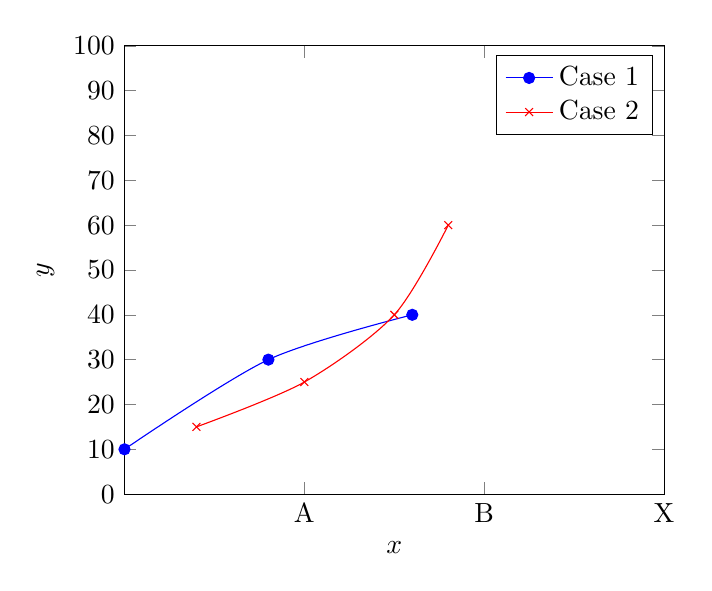
\begin{tikzpicture}
	\begin{axis}[
    	xlabel=$x$,
    	ylabel=$y$,
    	xmin=0, xmax=30,
    	ymin=0, ymax=100,
    	xtick={10,20,30},
    	xticklabels={A,B,X},   % <---
    	ytick={0,10,...,100}
            ]
		\addplot[smooth,mark=*,blue] 
			plot coordinates {
    			(0,10)
    			(8,30)
    			(16,40)
			};
		\addlegendentry{Case 1}

		\addplot[smooth,color=red,mark=x]
    		plot coordinates {
        		(4,15)
        		(10,25)
        		(15,40)
        		(18,60)
    		};
		\addlegendentry{Case 2}

	\end{axis}
\end{tikzpicture}

\printbibliography[omitnumbers=true,type=misc,heading=subbibliography,title={Online zdroje}]
%\printbibliography[omitnumbers=true,type=book,heading=subbibliography,title={Knižní zdroje}]
%\printbibliography[omitnumbers=true,type=article,heading=subbibliography,title={Články}]
%\printbibliography[omitnumbers=true,type=proceedings,heading=subbibliography,title={Zákony}]
%\printbibliography[omitnumbers=true,type=thesis,heading=subbibliography,title={Kvalifikační práce}]	
	
\end{document}